\section{Personalización de la interfaz gráfica}
\label{sec:gui_personalizacion}

Una vez que el pipeline de procesamiento multimedia estaba operativo y las funciones
principales del sistema eran estables, se abordó la transformación visual y operativa
de voctogui. La interfaz original presentaba un aspecto genérico, con fondo blanco
heredado del tema del sistema operativo y sin iconografía coherente. Esta personalización
se realizó de forma progresiva a lo largo del desarrollo, en paralelo a la incorporación
de nuevas funcionalidades, con el objetivo de convertirla en una herramienta de
producción profesional lista para su uso en eventos reales.

% ── Placeholder: captura de voctogui con tema oscuro y todas las funcionalidades ──
\begin{figure}[H]
  \centering
  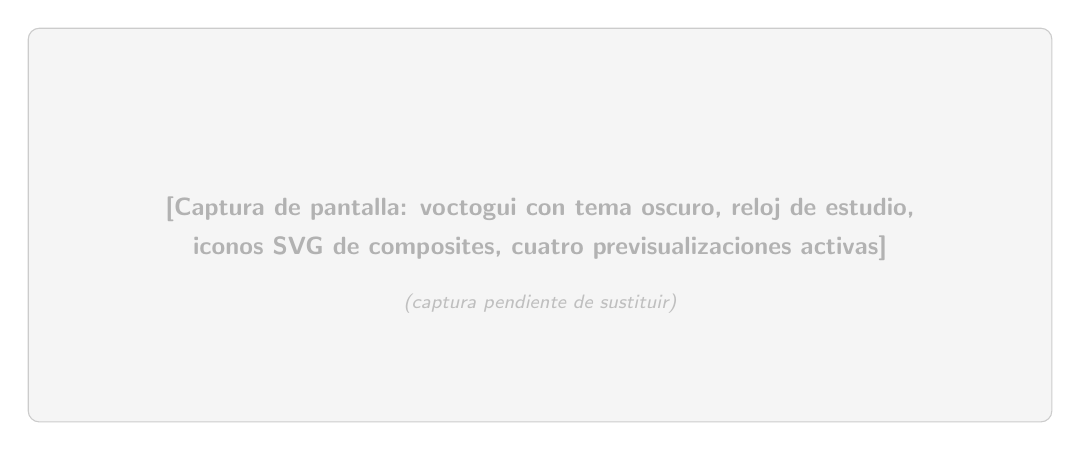
\begin{tikzpicture}
    \draw[rounded corners=4pt, fill=gray!8, draw=gray!40]
      (0,0) rectangle (13,5);
    \node[font=\sffamily\small\bfseries, text=gray!60] at (6.5,2.7)
      {[Captura de pantalla: voctogui con tema oscuro, reloj de estudio,};
    \node[font=\sffamily\small\bfseries, text=gray!60] at (6.5,2.2)
      {iconos SVG de composites, cuatro previsualizaciones activas]};
    \node[font=\sffamily\scriptsize\itshape, text=gray!50] at (6.5,1.5)
      {(captura pendiente de sustituir)};
  \end{tikzpicture}
  \caption[Interfaz gráfica voctogui personalizada]{Interfaz gráfica voctogui tras la
           personalización: tema oscuro CSS (\texttt{\#252a2c}), iconos SVG de
           composites, reloj de estudio y cuatro paneles de previsualización activos.}
  \label{fig:voctogui_personalizada}
\end{figure}

\subsection{Tema oscuro y hoja de estilos}

Se inyectó una hoja de estilos CSS (\texttt{voctogui.css}) que fuerza un fondo
\texttt{\#252a2c} y texto claro en todos los paneles. Los botones activos se iluminan
en amarillo (\texttt{\#ddbb00}), unificando el lenguaje visual de toda la interfaz y
proporcionando al realizador una retroalimentación visual inmediata sobre el estado
de cada control.

\subsection{Iconografía SVG}

Los botones de composite y de control de emisión se vincularon a iconos vectoriales
\texttt{.svg}, declarados en las secciones \texttt{[toolbar.composites]} y
\texttt{[toolbar.mix]} del fichero de configuración \texttt{default-config.ini}.
El uso de SVG garantiza que los iconos se escalan sin pérdida de calidad a cualquier
resolución de pantalla.

\subsection{Reloj de estudio}

Se integró el widget \texttt{StudioClock} en la parte inferior del panel de cámaras
mediante el diseño XML de la interfaz (\texttt{voctogui.ui}), envuelto en un
\texttt{GtkAspectFrame} para preservar las proporciones del panel de vídeo. El reloj
muestra la hora del sistema en tiempo real, indispensable para la coordinación de
escaleta en producciones en directo: el realizador puede sincronizar los cortes de
cámara con los tiempos marcados en el guión sin apartar la vista del monitor de
mezcla.

